\section{Material Analysis and Selection}
% % for code listings
% \begin{lstlisting}[style=cstyle, caption=System Architecture Code Example, label=lst:SystemArchitecture8]
% # Your code here
% \end{lstlisting}

% % for figures
% \begin{figure}[htbp] %h-ere t-op b-ottom p-page (separte) -good to allow all htbp to give the compiler more options
%     \centering
%     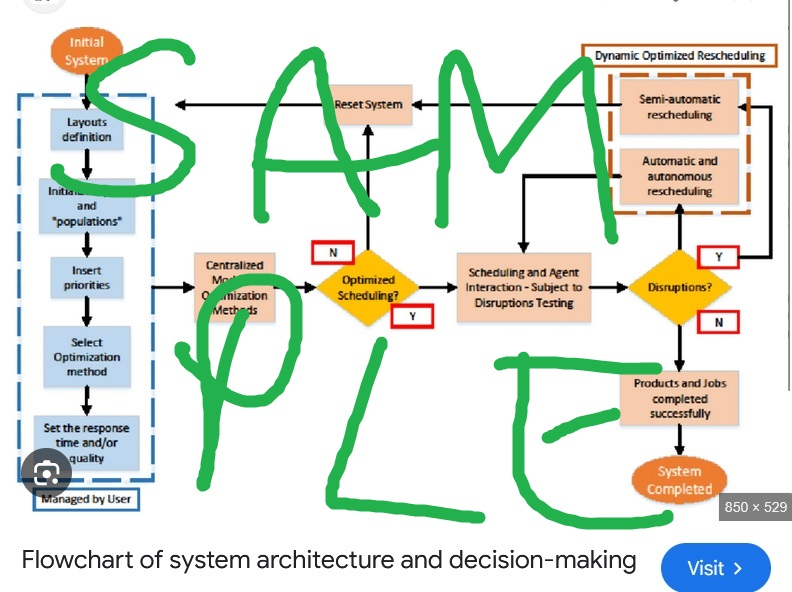
\includegraphics[width=0.6\textwidth]{figures/methodology/system_architecture.jpg}
%     \caption{System Architecture Diagram}
%     \label{fig:system-architecture3}
% \end{figure}

% % Include a flowchart in TEX mode
% \begin{figure}[H]
%     \centering
%     \scalebox{0.8}{ % Scale to 80% of original size
%         % try generating flowcharts as svg in Claude 
% and edit with inkscape instead of this.
% but claude did generate this one so might 
% be useful too but you can't easily make
% small repairs in inkscape


% CNN Transfer Learning Flowchart - Compact Multi-Column Layout
% \begin{figure}[htbp]

\centering
\resizebox{\textwidth}{!}{ % Scale to fit width while maintaining aspect ratio
\begin{tikzpicture}[node distance=0.8cm and 1.5cm, auto]
    % Define a smaller block style
    \tikzset{
      block/.style = {rectangle, draw, fill=blue!20, 
                      text width=7em, text centered, rounded corners, minimum height=1.8em, font=\small},
    }
    
    % Brazilian model training - Column 1
    \node [block] (brazildata) {Download Brazilian coins dataset};
    \node [block, below=of brazildata] (extract) {Extract dataset};
    \node [block, below=of extract] (setup) {Setup directories};
    \node [block, below=of setup] (define) {Define train/val dirs};
    \node [block, below=of define] (create) {Create CNN architecture};
    \node [block, below=of create] (compile) {Compile the CNN};
    \node [block, below=of compile] (train) {Train model};
    \node [block, below=of train] (trained) {Model trained (5 classes)};
    
    % Transfer learning - Column 2 (Middle)
    \node [block, right=2.5cm of brazildata] (freeze) {Freeze all layers};
    \node [block, below=of freeze] (replace) {Replace final layers};
    \node [block, below=of replace] (add) {Add regularization and dropout};
    \node [block, below=of add] (output) {New output layer (8 classes)};
    \node [block, below=of output] (finaltrain) {Train and fine-tune};
    \node [block, below=of finaltrain] (inference) {Perform inference on new coins};
    
    % UK data preparation - Column 3 (Right)
    \node [block, right=2.5cm of freeze] (ukdata) {Download UK coins dataset};
    \node [block, below=of ukdata] (ukextract) {Extract UK dataset};
    \node [block, below=of ukextract] (uksetup) {Setup UK directories};
    \node [block, below=of uksetup] (ukgen) {Create data generators (80/20 split)};
    
    % Connect all nodes with arrows
    \path [line] (brazildata) -- (extract);
    \path [line] (extract) -- (setup);
    \path [line] (setup) -- (define);
    \path [line] (define) -- (create);
    \path [line] (create) -- (compile);
    \path [line] (compile) -- (train);
    \path [line] (train) -- (trained);
    
    \path [line] (ukdata) -- (ukextract);
    \path [line] (ukextract) -- (uksetup);
    \path [line] (uksetup) -- (ukgen);
    
    % Connect the columns
    \path [line] (trained) -- node[midway, above] {Transfer} (freeze);
    \path [line] (ukgen) |- (finaltrain);
    
    % Connect middle column
    \path [line] (freeze) -- (replace);
    \path [line] (replace) -- (add);
    \path [line] (add) -- (output);
    \path [line] (output) -- (finaltrain);
    \path [line] (finaltrain) -- (inference);
    
    % Group boxes to show different stages with smaller padding
    \begin{pgfonlayer}{background}
        \node[group={[yshift=0.3cm]above:Brazilian Model Training}, fit={(brazildata) (extract) (setup) (define) (create) (compile) (train) (trained)}, inner sep=0.2cm] {};
        \node[group={[yshift=0.3cm]above:UK Data Preparation}, fit={(ukdata) (ukextract) (uksetup) (ukgen)}, inner sep=0.2cm] {};
        \node[group={[yshift=0.3cm]above:Transfer Learning}, fit={(freeze) (replace) (add) (output) (finaltrain) (inference)}, inner sep=0.2cm] {};
    \end{pgfonlayer}
\end{tikzpicture}
}
% \caption{CNN Transfer Learning Flowchart: Brazilian to UK Coins}
% \label{fig:cnn-flowchart}
% \end{figure} % \input is for tex files \includegraphics is for images
%     }
%     \caption{System Design Overview Flowchart}
%     \label{fig:decriptiveLabel22} % descriptive to call in text with \ref{fig:decriptiveLabel22}
% \end{figure}
\subsection{Material Selection and Requirements}
%add intro blurb here
The PCB will be operated in harsh environmental obstacles from strict 
requirements in both space and weight. PCB must withstand the extremities 
of immense pressures and vacuums, polarising temperatures, vibrations, 
impacts, space radiation and more. Generally, the materials for PCB made 
for space conditions are either polyimide or ceramic, as they can withstand 
extremely harsh conditions \cite{ABLcircuits}. Commonly materials used for 
space PCB include polyimide, PTFE and alumina \cite{CadenceDesignSystems2025}.

\subsection{External Factors}
%add intro blurb here
The PCB needs to sustain itself when it is launched into and deployed to 
outer space from the extreme heat it will experience from -200°C in the 
shadow of a celestial body to over 200°C when sunlight exposes on it 

\subsubsection{Extreme Temperature Variations}
Space exposes PCBs to extreme temperature fluctuations, which can affect 
their structural integrity and performance. Materials must maintain their 
thermal stability and dimensional consistency across a wide temperature range.

The temperature in space varies dramatically, ranging from extreme cold in 
the shadow of celestial bodies to scorching heat under direct solar exposure 
\cite{Proto-Electronics2024}. Materials expand and contract, with the magnitude 
of the dimensional change determined by the material's Coefficient of Thermal 
Expansion (CTE) \cite{911EDA2024}. When different materials in a PCB assembly 
have differing CTEs, the repeated cycles of expansion and contraction can result 
in considerable mechanical stresses at their interconnections \cite{Proto-Electronics2024}.

These stresses may result in severe failures such as solder joint cracking, 
PCB layer delamination, and even circuit malfunction \cite{Proto-Electronics2024}. 
As a result, materials with naturally low CTE values, such as ceramic PCBs, are 
widely used in space applications to reduce these concerns \cite{Proto-Electronics2024}. 
A material's capacity to resist multiple temperature cycles without degradation is 
also critical for long-term reliability in space missions \cite{resources.pcb.cadence}.


\subsubsection{Ionizing Radiation}
High-energy radiation, including cosmic rays, solar particles, X-rays, and 
UV radiation, exists throughout the space environment \cite{Proto-Electronics2024}.

This ionising radiation poses a significant risk to the performance and durability 
of electronic components, particularly those found on PCBs. Radiation exposure can 
impair semiconductor performance, potentially causing data corruption via bit flips 
and resulting in a steady loss of material properties with time \cite{Gatema2024}.

Celestial sources and the sun emit ionizing radiation that can disrupt the PCB's 
functionality and degrade the semiconductors' performance, hence, to protect the 
sensitive electronic components from being damaged by radiation, the PCBs must be 
made from radiation-hardened materials.

To mitigate these negative effects, radiation-hardened materials are frequently 
used in space-grade PCBs. Ceramic substrates, for example, are more resistant to 
radiation than many biological materials. Specialised coatings are also used to 
give another layer of protection to delicate electrical components \cite{Gatema2024}.

The use of materials with intrinsic radiation resistance is an important design 
concern for ensuring the ongoing operation of electronic devices in the harsh 
radiative environment of space \cite{PCBDirectory2025}.

\subsection{Internal Factors}
%add intro blurb here
\subsubsection{Mechanical Stresses}   
The PCB, housing and aperture will experience mechanical stresses during the launch 
and deployment in the spacecraft, from the vibrations generated from the launch and 
deployment phase it can cause structural damage. To mitigate this issue there are in 
place shock-absorbing mechanisms that include the PCB material being flexible and 
conformal coating to safeguard the electronic components' integrity. Flexible PCBs 
are more effective at absorbing disturbances and vibrations compared to rigid PCBs.

PCBs are subjected to immense mechanical strains throughout a space mission's launch 
and deployment phases. The tremendous vibrations and shocks produced during launch, 
along with the high gravitational forces experienced, can put great stress on every 
component of the PCB \cite{Proto-Electronics2024}.

Furthermore, the deployment of solar arrays and other spacecraft features may cause 
additional mechanical stress \cite{Proto-Electronics2024}. These forces can cause 
structural damage to PCBs, such as board cracking, layer delamination, and the 
breakdown of solder junctions that connect components \cite{Proto-Electronics2024}.

To address these issues, designers frequently use shock-absorbing mechanisms, such 
as flexible PCB materials like polyimide, which are more effective at absorbing 
vibrations than rigid counterparts. Conformal coatings are also used to give an 
extra layer of protection against physical damage during launch and deployment 
\cite{Proto-Electronics2024}. Furthermore, precise PCB layout design is required 
to guarantee a more even distribution of mechanical loads across the board 
\cite{Proto-Electronics2024}.

\subsubsection{Outgassing and Vacuum}


Outgassing is another internal factor which is when manufacturing the PCB, 
outgassing is a soldering wave defect that traps air within a PCB. This is 
a major issue as it can lead to the PCB impairment from the cavities or 
blowholes created by the air inside. This is often a result of defective 
manufacturing and poor material selection choices.

There is a strict size and weight limit for the PCBs because of the tight 
space in the spacecraft, thus the PCB must be compact and lightweight whilst 
maintaining equilibrium that it does neither compromise on the functionality 
and the structure of the PCB.

The near-perfect vacuum of space poses an additional notable challenge for 
PCB materials. Materials in this environment can undergo outgassing, which 
is the release of trapped volatile chemicals \cite{CadenceDesignSystems2025}. 
These outgassed compounds can have harmful impacts on delicate spacecraft 
equipment \cite{FSCircuits2025}. Optical instruments, such as cameras and 
telescopes, are especially susceptible to contamination by outgassed materials, 
which can deposit on their surfaces and degrade performance \cite{Proto-Electronics2024}. 
Similarly, thermal control surfaces can be influenced, affecting their ability 
to regulate the spacecraft's temperature \cite{911EDA2024}.

Furthermore, the release of gases near high-voltage components can raise the 
risk of corona discharge, which could hinder electronic operations and cause 
damage \cite{911EDA2024}. To address these difficulties, the materials used 
in space-grade PCBs must have low outgassing qualities. Polymers such as 
polyimide and PTFE (Teflon) are widely used because of their extremely low 
outgassing properties, which help to protect the integrity of sensitive 
spacecraft components and systems \cite{Proto-Electronics2024}.

\subsection{PCB Material Selection}  %2nd section of mat analysis section
%add intro blurb here

\subsubsection{High-Tg FR-4}
\begin{figure}[htbp]
    \centering
    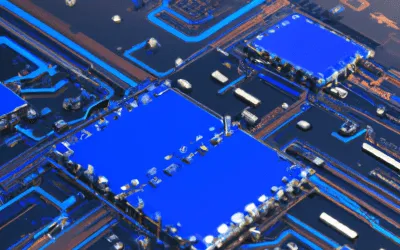
\includegraphics[width=10.5cm]{chapters/methodology/MaterialAnalysis/Fig1FRPCB.png}
    \caption{FR-4 PCB \cite{86PCB2024}}
    \label{fig:fr4-pcb}
\end{figure}

While not as extensively used as polyimide or ceramics in the most extreme space environments, high-Tg FR-4 laminates find application in scenarios where thermal conditions are less severe, such as within crewed spacecraft like the International Space Station \cite{CadenceDesignSystems2025}. 
These epoxy-based laminates possess a higher glass transition temperature (Tg) compared to conventional FR-4, providing greater stability at elevated temperatures.
Epoxy laminates typically have a glass transition temperature between 150-170°C \cite{CadenceDesignSystems2025}.

Using GRANTA EduPack 2022 R2, we found that FR-4 variations with dissipation factors (DF) of 0.015, 0.02, and more than 0.02 would be excluded from our nanosatellite PCB application. 
These materials were eliminated because they have larger signal losses at communication frequencies, reducing power efficiency in our power-constrained nanosatellite design.
The increased signal attenuation will compromise the reliability of data transmission and could also raise thermal loads on the board. Furthermore, ordinary FR-4 materials often have lower glass transition temperatures, which poses dimensional stability problems during the severe heat cycling encountered in the space environment (-60°C to +100°C). 
These restrictions would negatively impact both the electrical performance and long-term dependability of the PCB, making these materials unsuitable for the demanding circumstances of the space environment.

Even FR-4.0 with DF < 0.01, while superior to other FR-4 varieties, has limits for space applications.
Its glass transition temperature range (130-180°C) has a lower limit that may not be adequate for intense orbital thermal cycling.
Its thermal expansion coefficient and mild outgassing properties in vacuum may jeopardise long-term reliability and contaminate sensitive optical components.
Although more expensive, more specialised space-grade materials would be preferable for maximum performance in nanosatellite applications.

\subsubsection{Polyimide}
Research is conducted about materials suited for space PCBs, a prominent material used is Polyimide (PI), the common "space age" material with the highest performing class out of plastics.

Polyimide is a flexible polymer that is commonly used as a substrate material in space-grade printed circuit boards due to its inherent flexibility and lightweight nature \cite{CadenceDesignSystems2025}. 
This flexibility enables polyimide-based PCBs to effectively absorb mechanical stresses encountered during the dynamic stages of launch and spacecraft deployment.
Furthermore, polyimide has strong thermal stability, which allows it to survive temperature fluctuations in space to some extent \cite{CadenceDesignSystems2025}.
It also has low outgassing qualities, which are critical for avoiding contamination of sensitive spacecraft components \cite{Proto-Electronics2024}.
However, polyimide is generally regarded as less suited for applications involving high levels of radiation exposure than other materials such as ceramics \cite{CadenceDesignSystems2025}. 
For over three decades, DuPont's Pyralux laminates and Kapton polyimide films have been widely used in the aerospace and defence markets, with applications ranging from multi-layer insulation to wire wrapping and flexible circuit interconnects on solar panel backplanes \cite{MobilityEngineeringTech2024}. 
The Mars Rover Pathfinder also pioneered the use of adhesiveless laminate in space, using Pyralux AP material \cite{MobilityEngineeringTech2024}.

A material analysis was conducted using GRANTA Edupack and provides the general information about the material such as strengths and weakness shown in Appendix~\ref{appendix:material-analysis}. 
The main benefit of PI is that it has excellent heat resistance [260°C (500°F)] in continuous use, in tandem with having inherent fire-retardance and low smoke emission and excellent heat distortion temperature makes it a prime candidate for PCB. 
The limitations that Polyimide has is the high cost to produce, with the melt process being very difficult, making the manufacturing process of it be a slower process. 
It also has a relatively low impact strength, and worse elongation at break which can be a problem during the deployment process.

\subsubsection{Alumina}

\begin{figure}[htbp]
    \centering
    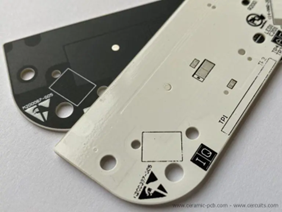
\includegraphics[width=7.5cm]{chapters/methodology/MaterialAnalysis/Fig2AluminaPCB.png}
    \caption{Alumina Oxide PCB \cite{CERCuits2025}}
    \label{fig:alumina-pcb}
\end{figure}
Alumina (Aluminium Oxide or Al$_2$O$_3$) is a ceramic that is a chemical compound of aluminium and oxygen, the 96\% refers to the purity of the aluminium.
A material analysis was also conducted using GRANTA Edupack and is shown in Appendix~\ref{appendix:material-analysis}. 
In abrasive environments they can maintain a long service life due to their high hardness and wear resistance, which would be ideal for the space usage because it has one of the extreme environments imaginable. 
They also have a high-temperature resistance with a high melting point at 2000-2100°C and outstanding thermal stability. 
It also has excellent corrosion resistance which is ideal for space usage where it can be a corrosive environment. 
It also is lightweight with its density ranging from 3.69 to 3.73 g/cm³. 
The disadvantages of it are the brittleness of the ceramic and can fracture on impact which limits the lifespan in the space usage to mechanical shocks. 
It is also difficult to machine from the high hardness so initial costs for manufacturing and lead time are higher than other materials \cite{mascera-tec}, \cite{Vhandy}.

\subsubsection{PTFE(Teflon)}

\begin{figure}[htbp]
    \centering
    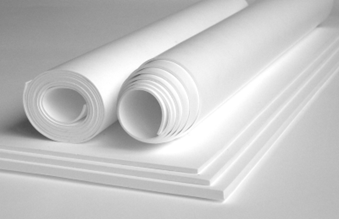
\includegraphics[width=9cm]{chapters/methodology/MaterialAnalysis/Fig3PTFE.png}
    \caption{PTFE/Teflon sheets \cite{Imimg2025}}
    \label{fig:ptfe-sheets}
\end{figure}

Polytetrafluoroethylene (PTFE) is a synthetic Fluoropolymer they have been known to be chemically inert, low friction properties and has a high heat resistant.

PTFE, also known as Teflon, is renowned for its great electrical characteristics, particularly its low loss tangent and dielectric constant \cite{CadenceDesignSystems2025}. 
These characteristics make it an excellent candidate for high-frequency applications, which are common in space communication systems \cite{CadenceDesignSystems2025}. 
Furthermore, PTFE is highly resistant to chemicals and outgassing, making it ideal for the hostile space environment \cite{CadenceDesignSystems2025}. 
Teflon is also used as a solid lubricant for numerous moving parts in spacecraft because of its resistance to heat and non-stick qualities \cite{FarrellLou2023}.

From the GRANTA Edupack it has a melting point that ranges from 315-339°C and can operates at its maximum service temperate from 250-270°C which allows the PCB to work in high temperature environments. 
Because it is chemically inert it is suitable for it to space PCB \cite{RayMingPCB2023}.

\subsubsection{Copper Foils}
\begin{figure}[htbp]
    \centering
    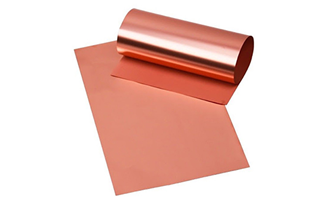
\includegraphics[width=8.7cm]{chapters/methodology/MaterialAnalysis/Fig4Copper.png}
    \caption{Copper foils \cite{ViinSolutions2022}}
    \label{fig:copper-foils}
\end{figure}

High-performance copper foils are essential in space-grade PCBs to ensure excellent signal integrity and efficient heat dissipation \cite{CadenceDesignSystems2025}. 
Copper's excellent electrical and thermal conductivity makes it the ideal material for conductive layers on a PCB. 
In applications requiring larger current carrying capability, thicker copper traces are frequently used \cite{SAEInternational2022}. 
The quality and thickness of the copper foil are crucial parameters that influence both the electrical performance and thermal management capabilities of the PCB in the demanding space environment.

\subsubsection{Kapton}

\begin{figure}[htbp]
    \centering
    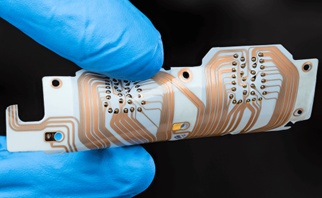
\includegraphics[width=8.5cm]{chapters/methodology/MaterialAnalysis/Fig5Kapton.png}
    \caption{Kapton PCB \cite{Goodfellow2025}}
    \label{fig:kapton-pcb}
\end{figure}

Kapton is highly radiation resistant and compatible with harsh conditions. 
Engineers typically use it to insulate cables and components in high vacuum chambers because it withstands radiation while having minimal influence on instrument base pressure \cite{MobilityEngineeringTech2024}. 
Kapton, which can withstand temperatures of up to 400°C, can be combined with other materials like gold to create heat-resistant blankets for use in spacecraft. 
Kapton's flexibility and outstanding performance under harsh temperatures make it an ideal material for a variety of insulation and protection applications in space hardware \cite{MobilityEngineeringTech2024}.


\subsubsection{Material Selection for PCB}
%%%%%%%%%%%%%%%%%%%%%%%%%%%%%%%%%%%%%%%%%%%%%%%%%%%%
The Comparing the elongation between the polyimide, alumina and PTFE, polyimide has the most ideal value being 75\%--80\% compared to alumina's 0.07\%-0.09\% or PTFE's 200\%-400\%, because having too little elongation can have a major risk of under deformation it will break, and having too much elongation causes the PCB to irreparably warp, having an in-between ensures it can deform when under forces without breaking.
Polyimide has the lowest density which is ideal for having weight limit on the shuttle craft. 
Polyimide has the highest cost per kg which can be a major restraint on the budget whilst alumina and PTFE are far cheaper in comparison. 
All 3 have the necessary operating temperature criteria of space temperatures from -200°C to +200°C. 
From this it is decided that the best material for PCB is polyimide, because it has the required strength, operating temperatures and it has the best middle road on its elongation (\%) and flexural modulus making it ideal for space usage.

\subsection{CubeSat Chassis Material} %3rd section of mat analysis section
The standard material that is used in the chassis of the CubeSat are aluminium alloys such as 6061 or 7075, which is to remain lightweight but without sacrificing strength. 
There's also need to thermal management to it to manage the fluctuations in space, commonly using multi-layer insulation to achieve this. 
The 4-digit designation represents what type of aluminium it is; the first digit can be 1 to 8 which represents which wrought it is. 
The second digit is often 0 meaning it is in the base form, any number other than this indicates it has been altered. 
The third and fourth digits identifies what individual alloys they are. 
A comparison table was created in GRANTA Edupack to compare all the Aluminium 6061 variants would be the best, and 6061-T651 was found to be the best out of all of them, as seen in the appendix.

\subsubsection{Aluminium 6061- T651}
Aluminium 6061-T651 has a good strength-to-weight ratio which offers a good balance between the strength and weight without compromising one to a detrimental degree. 
It's also strong with the tensile strength up to 320 MPa. 
It is used in many structural applications because it is strong by itself and is lighter than steel making it ideal in the automotive and aerospace industries. 
It is also highly recyclable and non-toxic so after usage it can be reused and does not cause harm to be in proximity with. 
It is also not suspectable to stress corrosion cracking making it ideal for space use when external and internal forces are applied towards it.

\subsubsection{Aluminium 7075}
Aluminium 7075 is one of the strongest aluminium available with a tensile strength listed at 580 MPa making it an ideal material for structural and load-bearing applications. 
Just like 6061 it is also lightweight with a good strength to weight ratio and highly recyclable. 
However, it is highly susceptible to stress corrosion cracking which is a major weakness especially for space applications from the external and internal forces applied to it.

\subsubsection{6061-T651 vs  7075}
In terms of strength Aluminium 7075 is considerably stronger than 6061, this makes 7075 a suitable material for applications requiring high strength such as Construction. 
However, 6061 is much more flexible with having better ductility making it easier to form weld into shape what the design requires. 
6061 also has better resistance in corrosion due to things in space such as atomic oxygen oxidising the metal. 
And 6061 is cheaper and simpler production process because of its machinability compared to 7075. 
It is decided that the most suitable for the chassis should be 6061-T651 because of the corrosion resistance, and machinability keeping cost down, with the better ductility to avoid the chassis structure to snap under forces, whilst 7075 is stronger, they already are suitable strength wise in space that it is a moot point.

\subsubsection{Emerging Materials and Future Trends} 
Emerging materials and future trends in space PCB technology are being shaped by advances in materials science and manufacturing techniques that try to solve the unique challenges provided by the space environment. 
Next-generation materials such as 2D materials, organic electronics, and metamaterials are being investigated for their potential to increase the performance and reliability of space electronics by offering severe temperature resistance, radiation shielding, and enhanced thermal conductivity \cite{Ona-Olapo2024}.

Furthermore, hybrid and composite materials, including self-healing polymers and multifunctional carbon fibre composites, are being developed to withstand the extreme conditions of space, such as micrometeorite impacts and electromagnetic interference, thus improving the feasibility and safety of space exploration \cite{Ince2023}. 
All these developments point to a future in which space PCB technology is more integrated, efficient, and capable of meeting the expanding demands of space missions.

\subsection{Quality Assurance and Reliability Standards in Space PCB Manufacturing}
%add intro blurb here

\subsubsection{NASA Standards}
NASA has comprehensive standards to ensure PCB quality and reliability PCBs used in space missions. 
NASA-STD-8739.1 defines the workmanship standards for polymeric applications on electrical assemblies, such as conformal coatings used to protect PCBs in defence and aerospace applications \cite{SCSCoatingSystems2021}. 
The Goddard Space Flight Centre (GSFC) has released GSFC-STD-8001, which specifies quality assurance standards for the design, procurement, fabrication, and use of high-reliability PCBs in GSFC project mission hardware \cite{GoddardSpaceFlightCentre2019}. 
GSFC-STD-8002 provides the requirements for the validation of manufacturing processes for printed wiring assemblies using water-soluble fluxes \cite{GoddardSpaceFlightCentre2015}. 
The NASA PCB Working Group (PCB WG) is a helpful resource, offering expertise in PCB technology assessment and recommendations for quality assurance measures \cite{CadenceDesignSystems2025}. 
NASA generally uses polyimide-based laminates with glass reinforcements in its PCB constructions \cite{CadenceDesignSystems2025}. 
The agency also emphasises the necessity of visual acuity testing in accordance with NASA-STD-8739.6 or IPC-QL-653, and PCB inspectors must hold IPC-A-600 Certified IPC Specialist (CIS) accreditation to ensure complete and accurate quality control \cite{GoddardSpaceFlightCentre2019}.
\subsubsection{ESA Standards}
The European Space Agency (ESA) also enforces strict requirements for materials and procedures used in space applications, including PCBs. 
These standards are extensively described in the European Cooperation for Space Standardisation (ECSS) series. 
ECSS-Q-ST-70-02C describes the thermal vacuum outgassing test protocols for screening space materials \cite{Leverett2024}. 
ECSS-Q-ST-70-10C specifies the requirements for qualified printed circuit boards \cite{ECSS2008}, whereas ECSS-Q-ST-70-60C Corrigendum 1 specifies the requirements for their procurement \cite{ECSS2019}. 
Other relevant ECSS standards address a wide range of materials, mechanical parts, and procedures, including cleaning, heat testing, soldering, and crimping \cite{ECSS2019}. 
These standards are intended to ensure the reliability and performance of electronic assemblies in the challenging space environment.

\subsubsection{IPC Standards}
IPC, a global trade group for the electronics industry, has established a number of standards that are commonly used in the production of space-grade PCBs. 
IPC-2221 is a generic standard that covers practically every area of PCB design \cite{CadenceDesignSystems2025}. 
Specific subsection standards are IPC-2222 for rigid boards, IPC-2223 for flex circuits, and IPC-2226 for HDI structures \cite{CadenceDesignSystems2025}. 
IPC-6012 specifies the certification and performance standards for rigid PCBs, whereas IPC-6013 accomplishes the same for flexible printed boards \cite{CadenceDesignSystems2025}. 
IPC-A-600 specifies the visual inspection standard for PCB acceptability \cite{CadenceDesignSystems2025}. 
For surface mount designs, IPC-7351 provides critical guidelines \cite{CadenceDesignSystems2025}.

For military and aerospace applications, IPC Class 3/A, as defined in IPC-6012 Class 3/A, denotes high reliability requirements \cite{SAEInternational2022}. 
Furthermore, the IPC 6012 Space Addendum specifies standards for class 3 boards used in the space and military avionics industries, including requirements to endure vibration, ground testing, and temperature cycling \cite{Shashikanth2021}.

\subsubsection{US Militarty Standards(MIL-SPEC)}
The United States Military has developed its own performance criteria for PCBs used in defence and aerospace applications. 
MIL-PRF-31032 specifies the requirements for high-reliability, stiff PCBs, whereas MIL-PRF-50884 addresses flexible PCBs \cite{RefWorks:leverett2024satellite}. 
MIL-PRF-55110 covers stiff PCBs used in military applications \cite{CadenceDesignSystems2024}. 
These standards set strict requirements on material selection, design, manufacturing processes, and testing to assure PCB dependability in hostile operating environments \cite{CadenceDesignSystems2024}. 
Furthermore, standards such as MIL-STD-810 explain environmental engineering issues for military equipment, while MIL-STD-461 establishes requirements for electromagnetic compatibility \cite{SAEInternational2022}. 
Compliance with MIL-SPEC standards is commonly required for PCBs used in military and aerospace systems.

